\section{Containers}
\subsection{Introduction}
\begin{frame}
  \frametitle{Containers}
  \begin{block}{Definition}
    A container holds a sequence of objects
  \end{block}
  \vfill
  \begin{block}{Two categories}
    \begin{itemize}
    \item Sequence containers: provide access to sequences of elements
    \item Associative containers: provide associative lookup based on a key
    \end{itemize}
  \end{block}
  \vfill
  \begin{block}{Associative containers}
    \begin{itemize}
    \item Ordered
    \item Unordered
    \end{itemize}
  \end{block}
\end{frame}

\subsection{Sequence containers}
\begin{frame}
  \frametitle{Sequence containers}
  \centering
  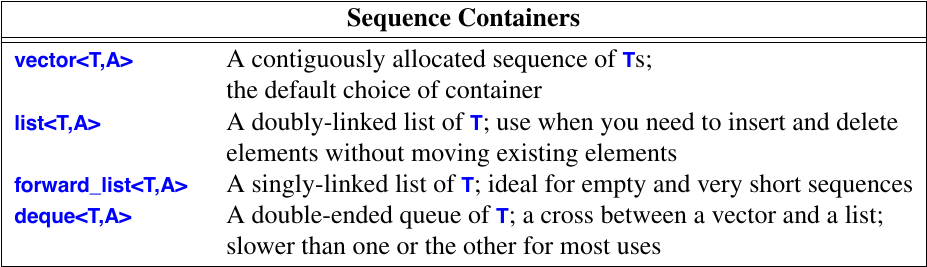
\includegraphics[width=\textwidth]{img/sequence_containers.png}
\end{frame}

\subsection{Associative containers}
\begin{frame}
  \frametitle{Ordered associative containers}
  \centering
  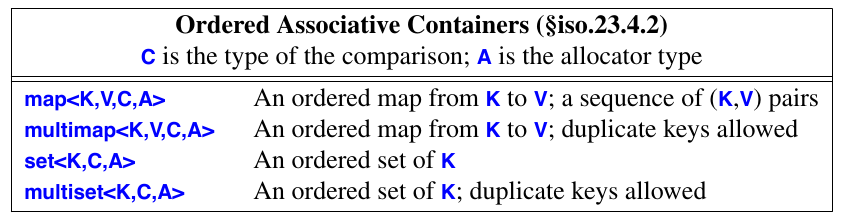
\includegraphics[width=\textwidth]{img/ordered.png}
\end{frame}
\begin{frame}
  \frametitle{Unordered associative containers}
  \centering
  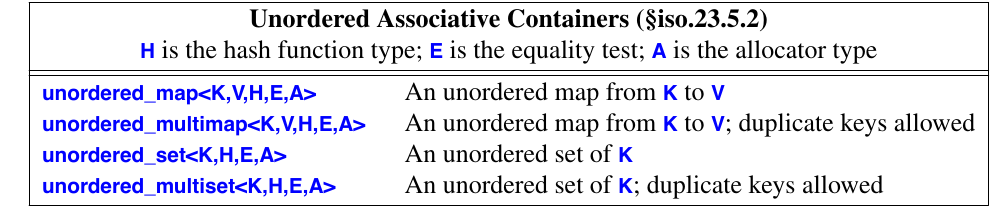
\includegraphics[width=\textwidth]{img/unordered.png}
\end{frame}

\subsection{Container representation}
\begin{frame}
  \frametitle{Array}
  \centering
  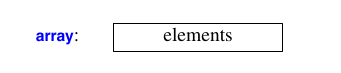
\includegraphics[width=0.5\textwidth]{img/array.png}
\end{frame}

\begin{frame}
  \frametitle{Vector}
  \centering
  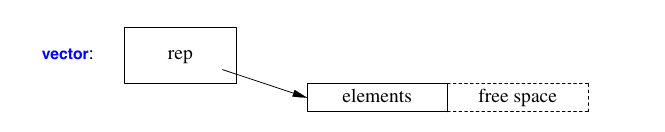
\includegraphics[width=\textwidth]{img/vector.png}
\end{frame}

\begin{frame}
  \frametitle{Forward list}
  \centering
  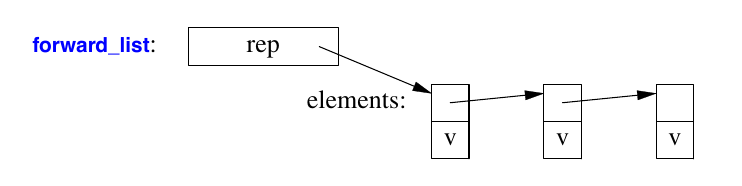
\includegraphics[width=\textwidth]{img/forward_list.png}
\end{frame}

\begin{frame}
  \frametitle{List}
  \centering
  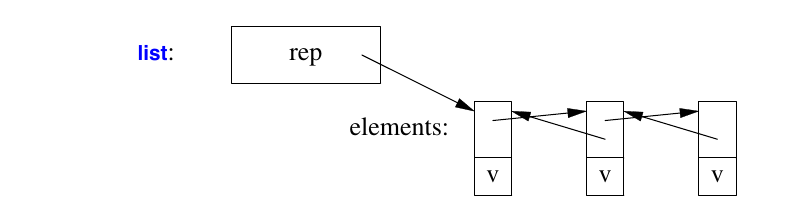
\includegraphics[width=\textwidth]{img/list.png}
\end{frame}

\begin{frame}
  \frametitle{Map}
  \centering
  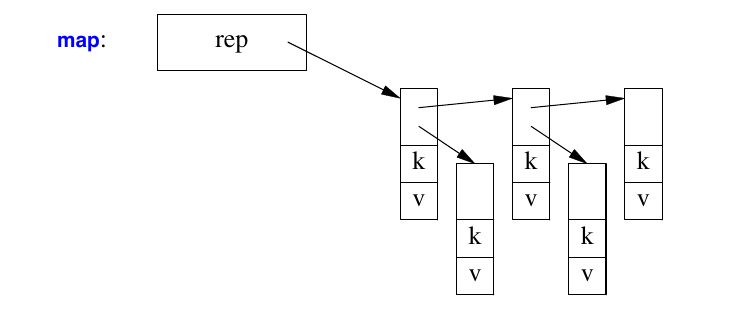
\includegraphics[width=\textwidth]{img/map.png}
\end{frame}

\begin{frame}
  \frametitle{Unordered map}
  \centering
  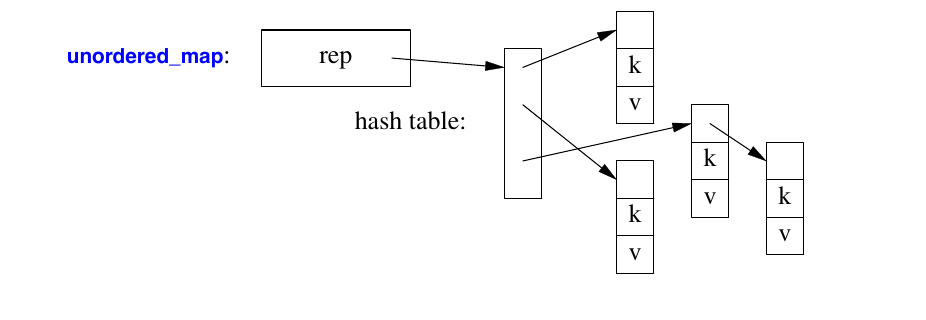
\includegraphics[width=\textwidth]{img/unordered_map.png}
\end{frame}

\subsection{Overview}
\begin{frame}
  \frametitle{Operations and types}
  \centering
  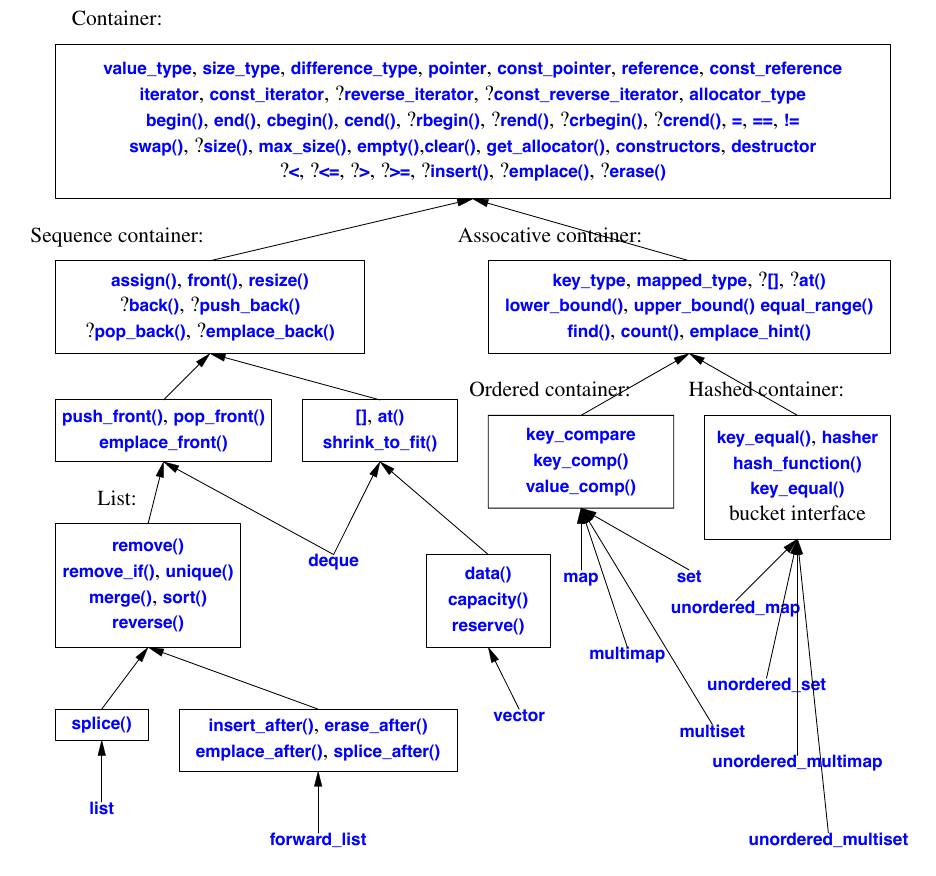
\includegraphics[height=0.95\textheight]{img/members.png}
\end{frame}

\begin{frame}
  \frametitle{Operation complexity}
  \centering
  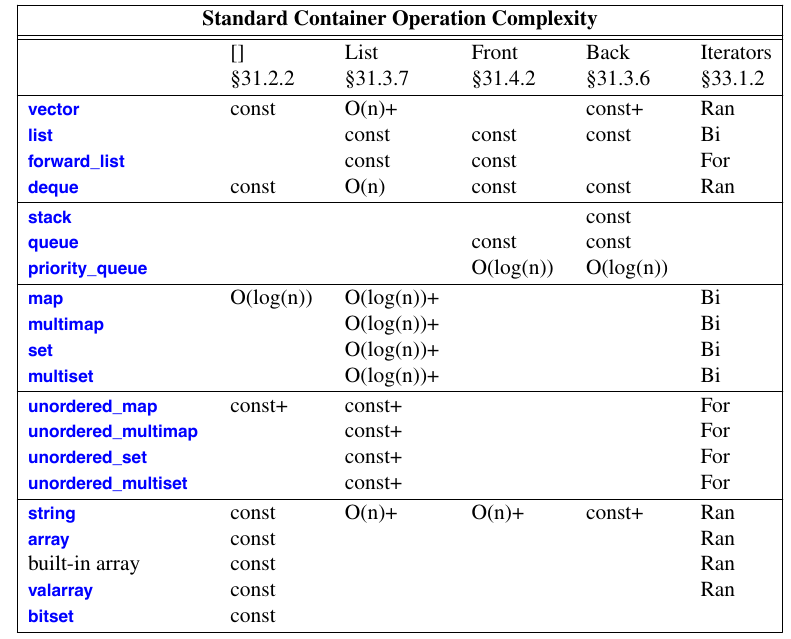
\includegraphics[height=0.9\textheight]{img/complexity.png}
\end{frame}

\subsection{Examples}
\begin{frame}[fragile]
  \frametitle{Prime numbers}
\begin{lstlisting}
#include <vector>

int main(){
  std::vector<int> primes;
  
  primes.emplace_back(2);

  for (int i=3; i<=max; ++i)
    if (is_prime(i))
      primes.emplace_back(i);

  for (const auto& x: primes)
    std::cout << x << std::endl;
}
\end{lstlisting}
\end{frame}

\begin{frame}[fragile]
  \frametitle{Word count}
\begin{lstlisting}
#include <map>
  
int main(){
  std::map<std::string, int> words;
  
  for (std::string s; std::cin>>s;)
    ++words[s];

  for (const auto& x: words)
  std::cout << x.first << ": "
            << x.second << std::endl;
}
\end{lstlisting}
\end{frame}

\begin{frame}[fragile]
  \frametitle{Word count}
\begin{lstlisting}
#include <unordered_map>
  
int main(){
  std::unordered_map<std::string, int> words;
  
  for (std::string s; std::cin>>s;)
    ++words[s];

  for (const auto& x: words)
  std::cout << x.first << ": "
            << x.second << std::endl;
}
\end{lstlisting}
\end{frame}
